
%What is eels?
%Sample experimental setup
%Sample spectra
%Signal types
%usages
%pros, cons/ STEM TEM
\setcitestyle{numbers,open={[},close={]}}


The focus of this work lies in  first principle theoretical calculations of EELS calculations, designed to be performed without experimental input.  However, new theoretical techniques must be validated through comparison to experiment.  To this end, this chapter presents an overview of experimental electron microscopy and  energy loss spectroscopy (EELS) before discussing the basics of first principles calculations. The chapter concludes with a review of the various methods used to calculate EELS theoretically.  The particularities of lithium materials are discussed at each step of this process.  
 
\section{Electron Energy Loss Spectroscopy (EELS)}

\subsection{Electron Microscopy}
The drive to improve battery materials relies on characterizing  nano scale features which define their properties \cite{goldstein_electron_2003}.  At these length scales, even state of the art optical light microscopes lack the resolution to discern these features \cite{rust_sub-diffraction-limit_2006}.  This limitation is due to the fact that nano scale features fall well below the diffraction limit of such microscopes, given by \cite{hecht}: 

\begin{equation}
	d = \frac{\lambda}{2n\textrm{ sin}(\theta)}
\end{equation}

Where n is the refractive index and d is the smallest distance between two discernible objects. For optical light ($\lambda$ = 400-800nm), it is impossible to routinely achieve the desired resolution ($\sim$ 1-50 nm) for characterization \cite{rust_sub-diffraction-limit_2006}.  Electrons however, have a wavelength dictated by \cite{goldstein_electron_2003}: 
\begin{equation}
 \lambda = \frac{h}{\sqrt{2 m_0 e E}}
\end{equation}
Where $h$ is Planck's constant, $m_0$, $e$ and $E$ are the rest mass, charge and energy of an electron.  In an electron microscope, electrons are accelerated to energies in the order of 1-100 keV giving them wavelengths in the range from 1-100 pm ($1\mathrm{pm}=10^{-12}$m), far  smaller than the distances between atoms ($\sim$0.5 nm) \cite{morales_laser_1998}.  Electron microscopes can therefore achieve a far lower theoretical diffraction limit  and are in fact currently limited by the technological constraints of the electron  lenses \cite{goldstein_electron_2003}.  This high resolution has made electron microscopy a key part of investigating material microstructure and is compared to other methods  in Fig \ref{method_scales} \cite{inkson_2_2016}. \\


\begin{figure}
	\centering
	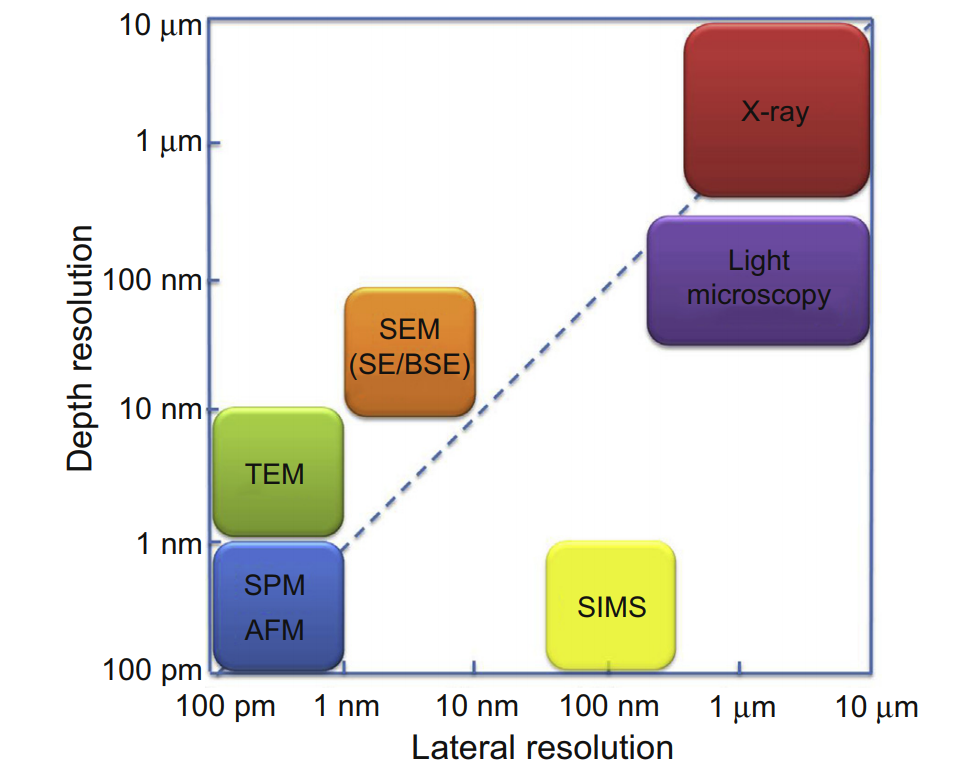
\includegraphics[width=0.7\textwidth]{method_scales}
	\caption{Resolution achievable by various techniques including Transmission and Scanning electron microscopy (TEM/SEM) and light microscopy, on a log-log scale.  Taken from Inkson, 2016 \cite{inkson_2_2016}.}
	\label{method_scales}
	
\end{figure}


In order to obtain images using electrons, electron microscopes use magnetic lenses to focus a beam of high energy electrons onto a sample, and collect the assorted types of signals resulting from the interaction, see Fig \ref{em_diagram}.\\


\begin{figure}
\begin{subfigure}{0.45\textwidth}
	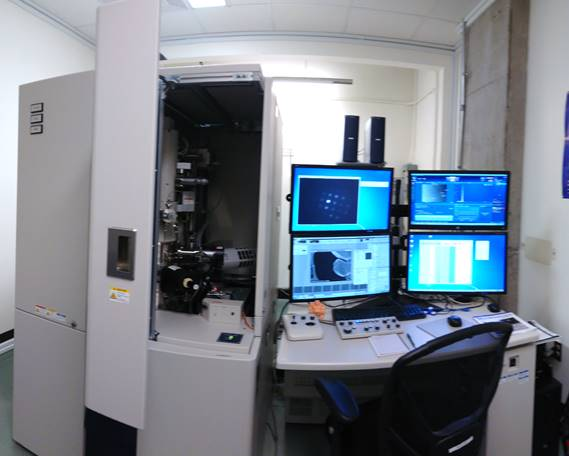
\includegraphics[width=1\textwidth]{SU_9000}
	\caption{}
\end{subfigure}
\hspace{0.05cm}
\begin{subfigure}{0.45\textwidth}
	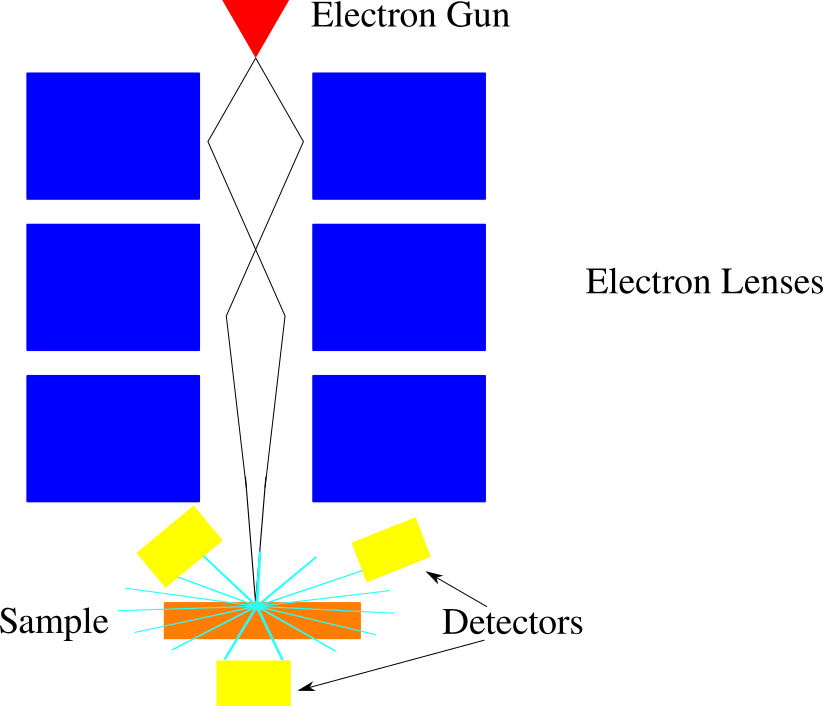
\includegraphics[width=1\textwidth]{EM_diagram}
	\caption{}
\end{subfigure}
	\caption{Example of an electron microscope (a) and working principles behind data acquisition (b). }
	\label{em_diagram}
\end{figure}

The large number of different signals generated when the electron beam interacts with a sample, (depicted in Fig \ref{specimen_emmisions}), can be used to perform a multitude of types of analysis \cite{williams_transmission_2008}.  A full discussion of the analysis methods at the disposal of electron microscopes is beyond the scope of this work and has been well documented elsewhere \cite{goldstein_electron_2003,Egerton,williams_transmission_2008,reimer_electron_1998}.  Instead, this discussion is limited to electron energy loss spectroscopy (EELS).  EELS is an electron microscopy technique that analyzes the transmitted inelastically scattered electrons, Fig \ref{specimen_emmisions}\cite{Egerton}.  It is mainly an analytic technique, however it is also possible to perform imaging with EELS \cite{varela_stem-eels_2012}.  EELS consists of collecting electrons that have passed entirely through the sample and binning them according to how much energy each one has lost, resulting in a spectrum such as shown in Fig \ref{EELS_spectra}.  The numerous distinct features arise from the various mechanisms through which beam electrons can lose energy in the sample.  Each mechanism results in a particular feature in the spectrum, of which the main ones are described below:
\begin{figure}
	\centering
	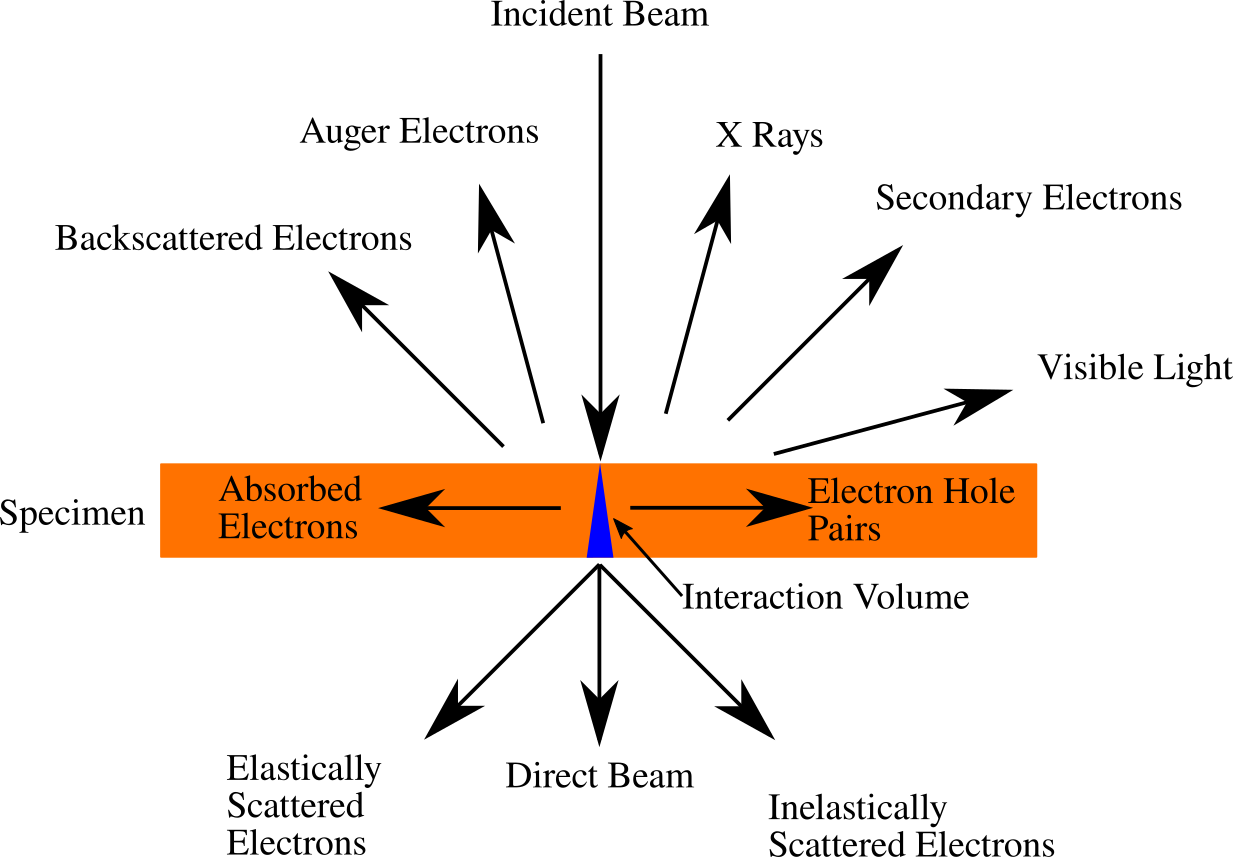
\includegraphics[width=0.65\textwidth]{specimen_emmisions.png}
	\caption{The numerous types of signals emitted when an electron beam encounters a sample in an electron microscope.   Redrawn from Williams and Carter 2008 \cite{williams_transmission_2008}.  }
	\label{specimen_emmisions}
\end{figure}

\begin{figure}
	\centering
	
\includegraphics[width=0.75\textwidth]{EELS_spectra.png}
	\caption{Sample EELS spectra identifying the main features, the zero loss peak, plasmon peak and ionization edges with fine structure.   The intensities are on a log scale, and span approximately 6 orders of magnitude between the zero loss and the ionization edges.  }
	\label{EELS_spectra}
\end{figure}

\begin{itemize}
	\item \textbf{Zero Loss Peak (ZLP):} The majority of the electrons in EELS pass through the specimen without experiencing an inelastic interaction, and retain their initial energy.  The width of the ZLP defines the resolution of the spectrum and is due to energy spreading as the beam passes through the electron lenses \cite{colliex_illustrated_1985}.  For thin samples, the ZLP is also the most intense feature on a spectrum \cite{Egerton}.  
	
	\item  \textbf{Background:} Beam electrons can excite loosely bound electrons close to the Fermi level into the unoccupied conduction band.  Due to the large number of possible transitions and the fact that high energy events are less favourable, this results in a smoothly decaying background \cite{Egerton}.
	
	\item \textbf{Plasmon Peak:}  The electron beam can excite multiple atoms in a solid collectively, creating a wavelike oscillation in the electron cloud of the solid \cite{Egerton}.  These are called plasmon excitations and result in a peak appearing between 5eV-30eV \cite{Egerton}.  The shape and intensity of the plasmon peak is dependent on the bond strength of the material and can be used to probe properties such as thickness and surface topology \cite{malis_eels_1988,nelayah_mapping_2007}. 
	
	\item \textbf{Ionization Edges:} Beam electrons can excite core electrons in a sample to the conduction band.  As an atom's core states are in general, isolated from its surroundings, the ``edges" for each element will occur at specific energy locations, independent of sample, analogous to characteristic x-rays \cite{Egerton}. These can be used to determine sample composition \cite{Egerton}.  
	
	
	
\end{itemize}
 

The array of independent interaction mechanisms occuring in EELS opens the possibility of beam electrons undergoing multiple inelastic events in the sample, referred to as plural scattering.  In order for meaningful data to be extracted from a spectra, plural scattering must be minimized \cite{Egerton}. This is achieved by using samples thinner or at least comparable to the path length of the beam electrons \cite{Egerton}.  If samples are too thick, duplicate plasmon peaks appear which  drown out the relatively weaker ionization edges see Fig \ref{multiple_plasmons}.   Consequently, samples must be made thin enough to analyze the more sensitive parts of EELS spectra, amongst others near edge structure. \\

\begin{figure}
	\centering
	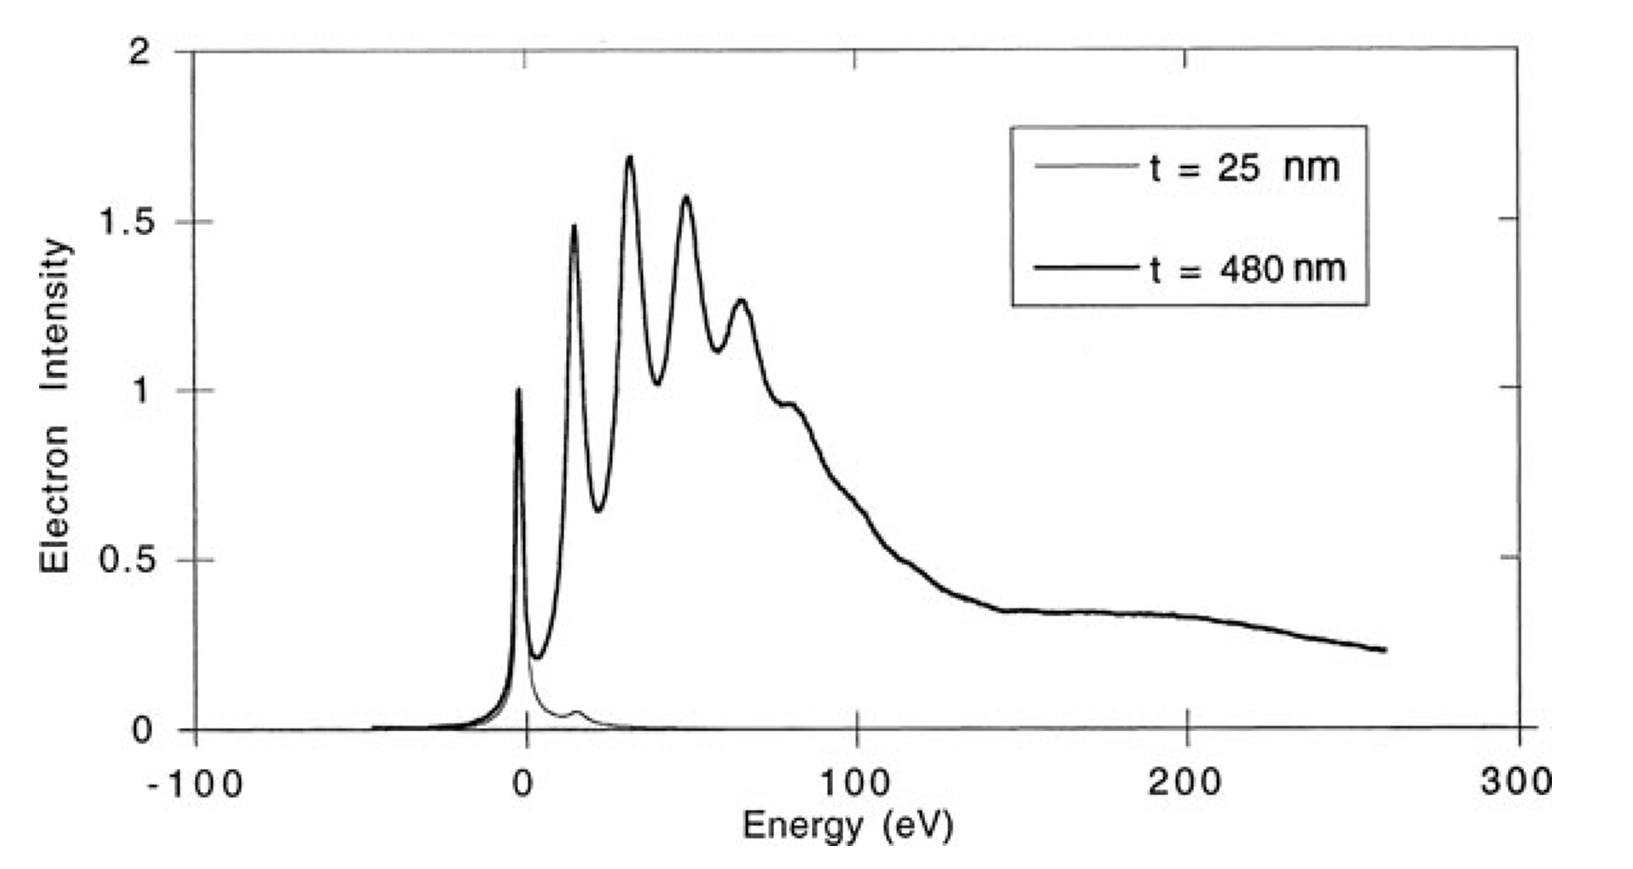
\includegraphics[width=0.75\textwidth]{multiple_plasmons.png}
	\caption{Two spectra demonstrating the importance of thin samples and single scattering events. In the thicker sample, plural scattering results in multiple evenly spaced plasmon peaks with  intensities larger than the zero loss extending well past 100eV.  The high background from the plasmon peaks and the thicker sample drown out any structure due to ionization edges \cite{Egerton}. Taken from Egerton, 2011 \cite{Egerton}.}
	\label{multiple_plasmons}
\end{figure}





\subsubsection{Near Edge Structure}
Ionization edges in EELS possess features extending up 50 eV beyond the onset of the edge, referred to as energy loss near edge structure (ELNES) \cite{Egerton}.   These features are a reflection of the unoccupied states in the conduction band that represent the final states available to sample electrons.  The band structure of the conduction band is largely dependent on the local bonds of the atom in question.  Because of this, ELNES can be used to investigate properties dependent on the local environment of each element.   Crystal structure is one such property, and ELNES can be used to distinguish different crystal structures of the same element such as carbon in graphite vs diamond, see Fig \ref{carbon-k-edge} \cite{hamon_elnes_2004}.  ELNES is also sensitive to impurities or dopants that would effect the band structure \cite{torrisi_atomic_2016}.  The large decay in intensity with increasing energy seen in Figure \ref{EELS_spectra}, limits the useful range ionization edges to those less than $\sim$2keV which corresponds to approximately the K edge of silicon (Z=14) \cite{reimer_transmission_2008}.  The relatively small intensity of ELNES make their analysis highly dependent on the experimental setup, which is discussed in the following section.  \\


\begin{figure}
	\centering
	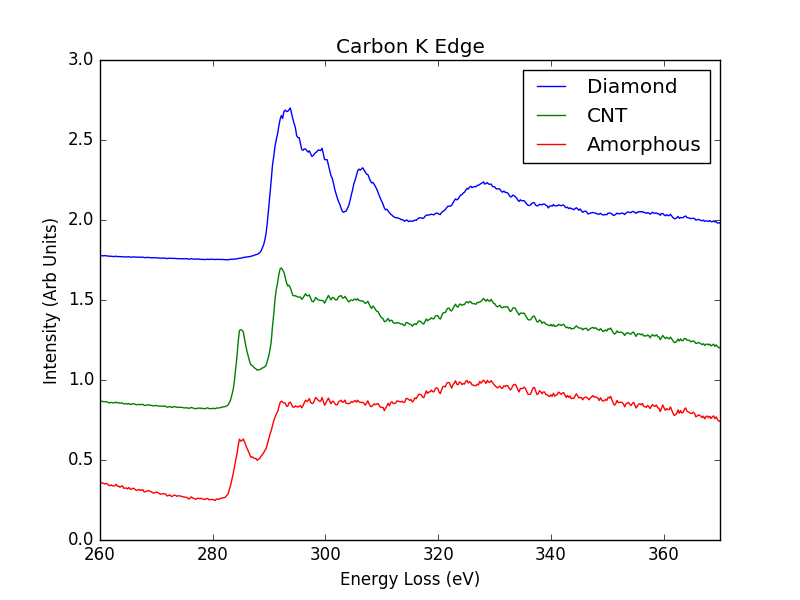
\includegraphics[width=0.75\textwidth]{Carbon_k_edges}
	\caption{Carbon K edge taken at 30keV at McGill. The different crystal structures (diamond, carbon nanotube, and amorphous) result in distinctly different ELNES which can be used for identification. The spectra have separated with a vertical offset to facilitate comparison. }
	\label{carbon-k-edge}
\end{figure}


\subsection{EELS in Experiment}

In order to collect EELS spectra, electrons must pass entirely through the sample, making EELS a technique for transmission electron microscopes (TEM's)\cite{Egerton}. In order to collect these transmitted electrons and divide them according to energy, a magnetic prism is placed below the specimen to redirect the electrons into a detector,  Fig \ref{prism}.  Inside the magnetic prism, there is a $\mathrm{\textbf{B}}$ field perpendicular to the beam direction which exposes the transmitted electrons to a Lorentz force (bold text indicates vector quantities) \cite{griffiths_em}: 


\begin{equation}
	\textbf{F}_B = q (\textbf{v} \times \textbf{B})
\end{equation}

As the force varies according to the velocity of the electrons, the magnetic prism  separates the electrons according to their energy: 

\begin{gather}
\textbf{F}_B = e (\textbf{v} \times \textbf{B}) =  \frac{m \textbf{v}^2}{\textbf{r}} = \textbf{F}_c \\
 r =  \frac{mv}{eB} = \frac{\sqrt{2mE}}{eB}
\end{gather}

\begin{figure}
 \centering
 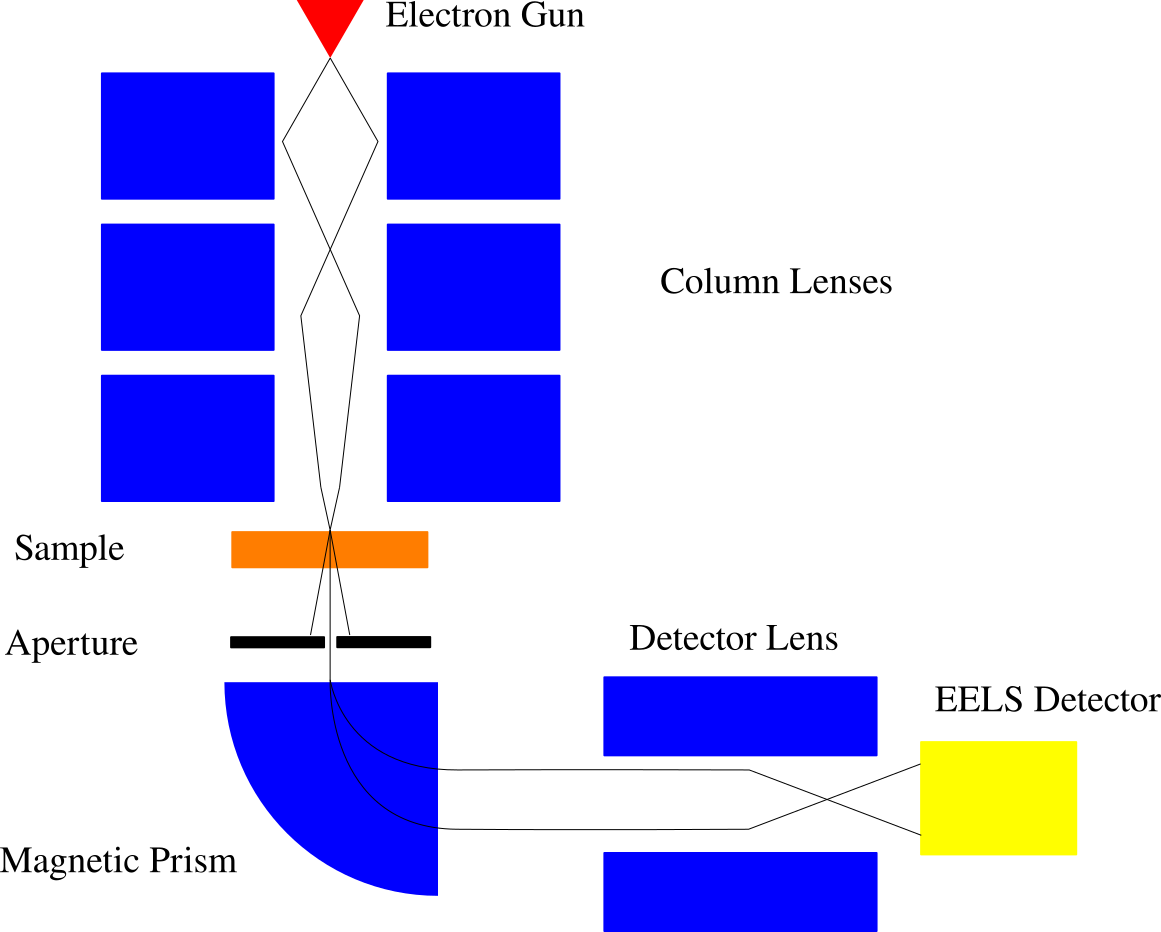
\includegraphics[width=0.75\textwidth]{Expt_setup.png}
 \caption{Experimental EELS setup, with the various magnetic lenses depicted in blue.  }
 \label{prism}
 
\end{figure}

Where  $E$ is the energy of each electron after passing through the sample.  Spectra are obtained by mapping each location on the detector to a corresponding energy loss value. Images are produced by  rastering the beam over the sample and using the intensities of a specific energy loss value to create an image.\\ 

The quality of EELS results depends numerous factors in the microscope.  Foremost among these are properties of the electron beam.  In order to obtain accurate results with regards to the finer features, the beam electrons must have very similar energies before striking the sample, within a few eV.  The larger this spread ($ \delta E $), the worse the energy resolution on the sample which obscures features in ELNES.  The energy spread is largely dictated by the electron gun, with the choice for EELS being a field emission gun ($\delta E \sim 0.5-1eV$), as older style tungsten and LaB$_6$ guns are unsuitable for EELS with energy spreads greater than 2 eV \cite{reimer_transmission_2008}.  The energy resolution can be further improved to the order of $\sim$10meV through the use of monochromators \cite{hachtel_exploring_2018}.  This improved energy resolution however comes at the cost of beam current which is another essential parameter for performing EELS.  This is because sufficient signal needs to be collected to render the statistical $\sqrt{N}$ errors small enough for features to become discernible.  At higher energies, introducing a monochromators can results in a trade off between experimental error from the beam and statistical errors due to lack of counts.  Lower current also translates into longer acquisition times, which expose the sample to more beam damage.  In addition to the beam properties, EELS results also depend largely on the imaging mode being used in the electron microscope as is discussed below.


\subsubsection{TEM vs SEM EELS}
There are two main branches of electron microscopy: scanning electron microscopy (SEM) and transmission electron microscopy (TEM).  TEM typically operates with beam energies between 100-300 keV designed to penetrate through thin samples, while SEM operates between 1-30 keV targeted towards analyzing bulk samples.  Each method has its own advantages.  The thin samples in TEM's result in a minimal interaction volume, far higher spatial resolution and have the ability to image individual atoms \cite{hansen_atomic-resolution_2001}. SEM's are optimized to scan the surfaces of samples and the large interaction volumes allow them to analyze bulk properties.  SEM is also a more economical and flexible tool as it has far fewer sample requirements.   EELS has been conventionally performed in TEM's as it requires the beam to pass through the sample and higher beam energies allow for thicker samples. Recent advances however have allowed EELS to be performed using an SEM with accelerating voltages of 30 keV \cite{SU_9000}.  As in a TEM, EELS in an SEM at 30keV requires thin samples, but offers the advantage of reducing the beam damage which has been essential for investigating lithium materials. 



\subsection{Lithium in EELS}
Lithium materials present a number of challenges to EELS analysis.  Lithium ion battery materials are in general semiconductors with band gaps of varying sizes. Coupled with lithium's highly mobile nature, lithium materials are highly sensitive to electron beam damage.  When performing analysis, damage results from the charge buildup when an electron beam passes through a sample.  In electron conductive samples (eg. metals), this charge can be dissipated to some extent, however in materials with a band gap (eg. insulators, battery cathodes), the charge can displace lithium ions and break down the crystal structure.  Lithium's high mobility also makes it vulnerable to knock on damage.  This effect occurs when an electron interacts inelastically with an atom's nucleus and results in sufficient momentum transfer to displace it from its lattice site.  Lithium is particularly vulnerable to this interaction because it requires only a small amount of energy ($ \sim 0.2-3$eV) to displace it through a crystal \cite{kang_factors_2006}.  Lithium's sensitivity to the beam make EELS's short acquisition times, on the order of seconds, well suited for its analysis. Recent developments enabling EELS at 30keV have made it applicable to a new range of lithium materials.\\  

Beyond the experimental essentials, EELS analysis of lithium materials is further complicated by lithium's only ionization edge being located around 55eV.  55eV is at the boundary of what is considered reasonable for analysis as it lies close to the plasmon peak. The decay of the plasmon peak complicates background subtraction and makes it highly vulnerable to sample thickness and plural scattering.  This energy range also often results in overlap between the lithium K-edge and the $\mathrm{M_{2 / 3}}$ and $\mathrm{M_4}$ edges of transition metals. In particular, the edges of Mn, Fe and Ni, all fall between 40-70eV.  As these elements are key components to cathode materials, they can require further steps for analysis to be possible.



\subsection{Preprocessing}

There are two key steps to be performed upon acquiring an ELNES spectra before it can be used for meaningful conclusions, background subtraction and deconvolution. 





\subsubsection{Background Subtraction} \label{bg_section}
The smooth decaying background in EELS spectra needs to be removed in order to isolate and analyze ELNES.  However, the EELS background does not decay at a fixed rate and varies with energy and based on the presence of edges \cite{new_bg}. Consequently, it is not possible to fit a single function to an entire spectrum.  Instead, the method of choice relies on fitting to a window directly before an ionization edge and refitting for each edge as needed.  The most prevalent function used for this purpose is a power law decay \cite{Egerton}: 

\begin{equation}
	I_{bg} = AE^{-r}
\end{equation}


Where $E$ is the energy loss and $A$ and $r$ are fitting factors, typically determined through a least squares procedure \cite{reimer_transmission_2008}.  This method has limitations due to different regions of the spectra decaying at different rates, with $r$ ranging from 2 to 6.5 \cite{reimer_transmission_2008}. A fit must therefore be performed for every feature being analyzed in a spectrum \cite{verbeeck_model_2004, egerton_inelastic_1975}.  A downside of this method is the dependency on the size and location of the fitting window which results in instability in the fits, as shown in Fig \ref{bg_removal}.  Difficulty in removing the background is further complicated in situations when edges overlap or when attempting quantitative analysis.  Coupled with the instability of power law fitting, this has resulted in a number of alternate models, such as polynomials, being proposed for specific cases. The power law method however, remains the most prevalent \cite{verbeeck_model_2004, riedl_extraction_2006}.  

\begin{figure}[H]
	\centering
	\begin{subfigure}{0.45\textwidth}
		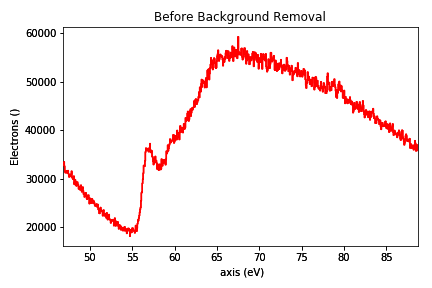
\includegraphics[width=1\textwidth]{full_bg.png} 
		\caption{}
		\label{full_bg}
	\end{subfigure}
	\hspace{-0.01cm}
	
	\begin{subfigure}{0.45\textwidth}
		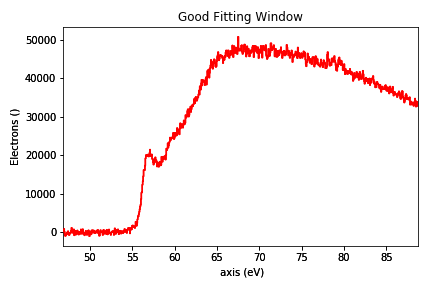
\includegraphics[width=1\textwidth]{good_window.png} 
		\caption{}
		\label{good_window}
	\end{subfigure}
	\begin{subfigure}{0.45\textwidth}
		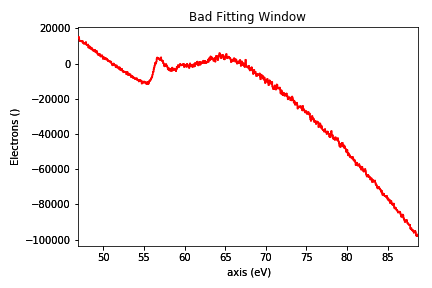
\includegraphics[width=1\textwidth]{bad_window.png} 
		\caption{}
		\label{bad_window}
	\end{subfigure}
	\caption{Results of power law background removal from raw spectrum (a) of metallic lithium K edge, using an appropriate (b)and inappropriate (c) window choices.}
	\label{bg_removal}
\end{figure}

\subsubsection{Deconvolution} \label{deconvolution}
Despite significant improvements in experimental equipment, there is still a degree of energy spread on beam electrons, typically in the range of $\sim$0.5-3eV.  This energy spread results in the observed ELNES on a spectra to be a convolution between the ``actual" ELNES and the ZLP.  Additionally, the probability plural scattering must also be addressed, as the low loss region of the spectrum is convoluted into the output spectra.  In order to recover the single scattering spectrum, the output must undergo deconvolution.  A number of techniques can be adopted for this purpose which can be split into either Fourier or Bayesian methods.   Fourier techniques rely on describing the signal as a number of convolutions:

\begin{equation}
 	J(E) = Z(E))\ast[\delta(E) + \frac{S(E)}{I_0} +  \frac{S(E) \ast S(E)}{2! I_0}   + ...]
\end{equation}



Where J(E) is the obtained spectra, Z(E) is the zero loss peak, S(E) is the single scattering spectra, and I$_0$ is the integrated intensity of the zero loss.  The double scattering term is the convolution of the two single scattering terms, weighted by the decreased probability according to Poisson statistics.   Taking a Fourier transform of this turns all of the convolutions into products: 

\begin{equation}
	j(\nu) = z(\nu) \left(1+\frac{s(\nu)}{I_0}+   \frac{s^2(\nu)}{2! I_0}+ \frac{s^3(\nu)}{3! I_0} + ...\right)
	\label{fourier_spectra}
\end{equation} 

Which can in turn be collapsed into an exponential:

\begin{equation}
	j(\nu) = z(\nu)\mathrm{exp}[s(\nu)/I_0]
\end{equation}

This equation can then be solved for $s(\nu)$ and reverse Fourier transformed to obtain the single scattering spectra.  In order to avoid amplifying the noise in the original spectra,  represented by high frequency terms in Fourier space, the result must be broadened by a modifier.  Thus, deconvolution can improve the energy resolution of the spectra only to a certain extent.  \\

More recently, Bayesian methods have found success as well, in particular the Richardson-Lucy technique \cite{richardson_lucy}. This technique is based on iterative methods initially developed in astronomy and used for the deconvolution of images, including those taken with the Hubble space telescope \cite{hubble}.  Similar to Fourier methods, the starting point is a convolution of the ideal spectra with the low loss, or point spread function ($R(E)$):

\begin{equation}
J(E) = R(E)\ast S(E)
\end{equation}

As an EELS spectra is inherently pixilated by the CCD, the convolution can be transformed into a sum, defining the observed intensity at a pixel based on the intensity of the surrounding pixels: 

\begin{equation}
	J(i) = \sum_{j} P(i,j) S(j)
\end{equation}
Where $P(i,j)$ defines how much the intensity at pixel $j$ affects pixel $i$.  
From here, the Richardson-Lucy algorithm applies Poisson statistics and iteratively calculates the single scattering spectra as  \cite{richardson_lucy}:  

\begin{equation}
S^{k+1}(j) = S^k(j) \left(\sum_{i} \frac{P(i,j)J(i)}{\sum_{l}P(i,l)S^k(l)}\right) \bigg/ \left( \sum_{i} P(i,j)\right)
\end{equation}

Where $k$ is the iteration number.  As with Fourier methods, the final spectra cannot gain any more information, and excessively increasing iterations results in increased noise and artifacts, this effect is demonstrated in Fig \ref{RL_iter}.  

\begin{figure}

	\begin{subfigure}{0.3 \textwidth}
		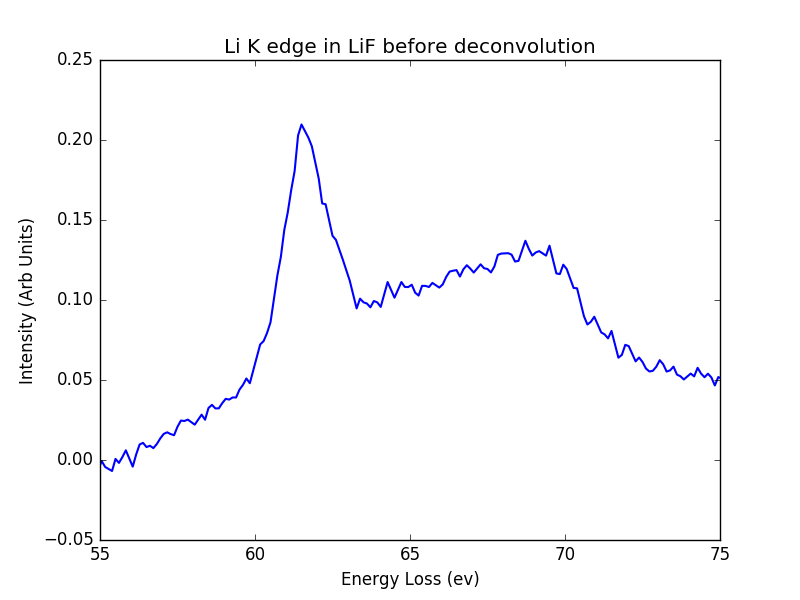
\includegraphics[scale=0.31]{/deconvolutions/0iter.png}
	\end{subfigure}
	\hfill
	\begin{subfigure}{0.3 \textwidth}
		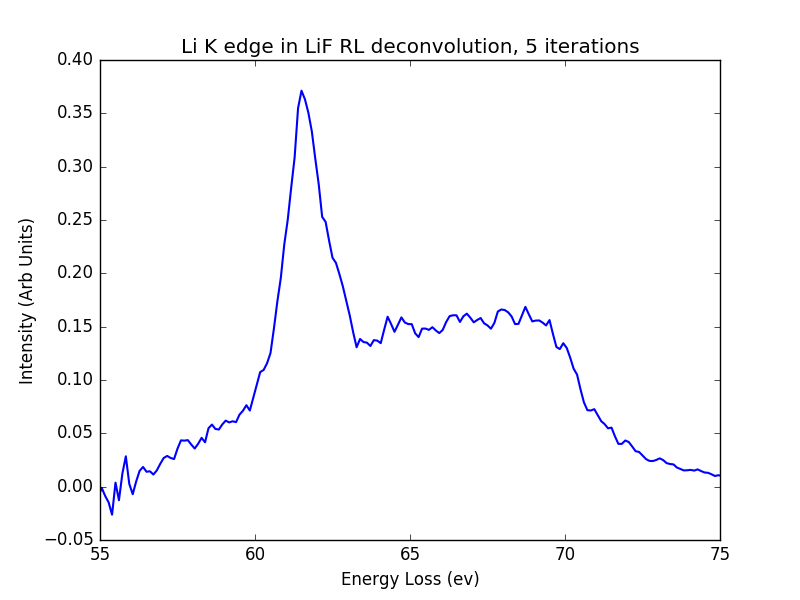
\includegraphics[scale=0.31]{/deconvolutions/5iter.png}
	\end{subfigure}
	\hfill
	\begin{subfigure}{0.3 \textwidth}
		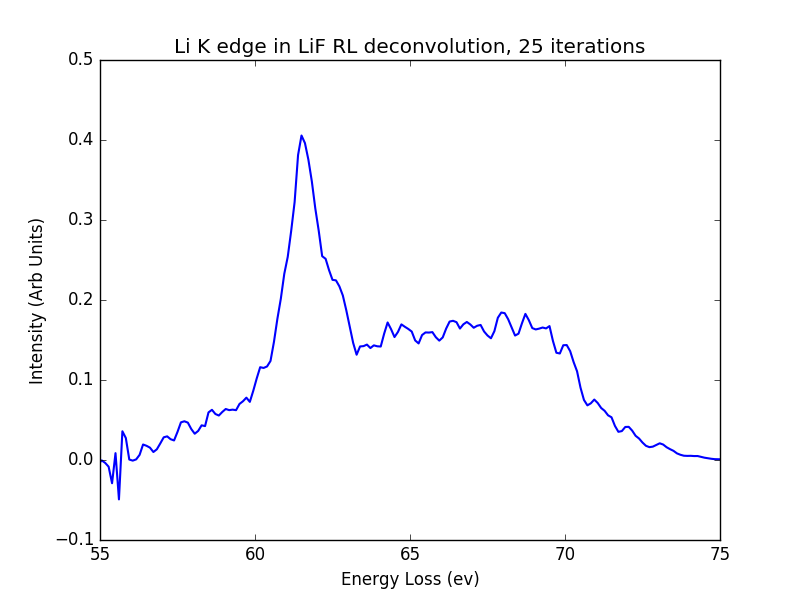
\includegraphics[scale=0.31]{/deconvolutions/25iter.png}
	\end{subfigure}
	\\
	\begin{subfigure}{0.33 \textwidth}
		
		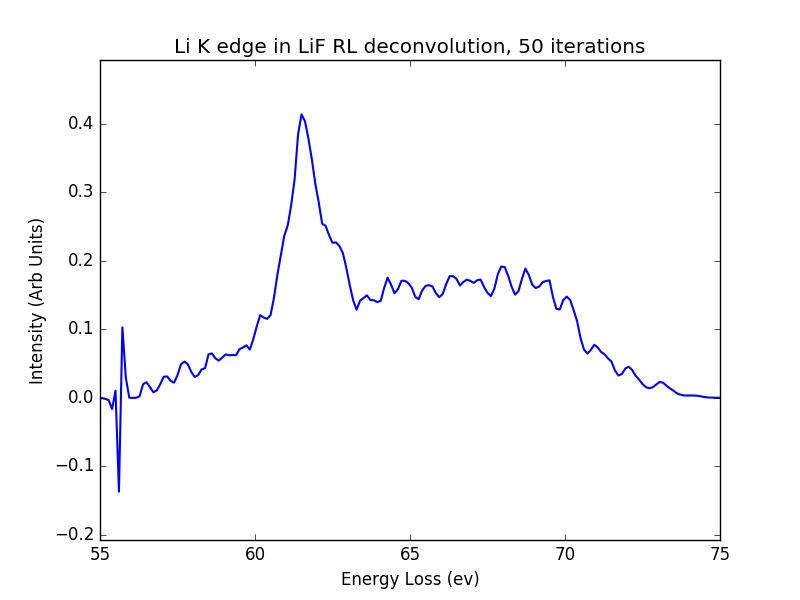
\includegraphics[scale=0.31]{/deconvolutions/50iter.png}
	\end{subfigure}
	~
	\begin{subfigure}{0.33 \textwidth}
		
		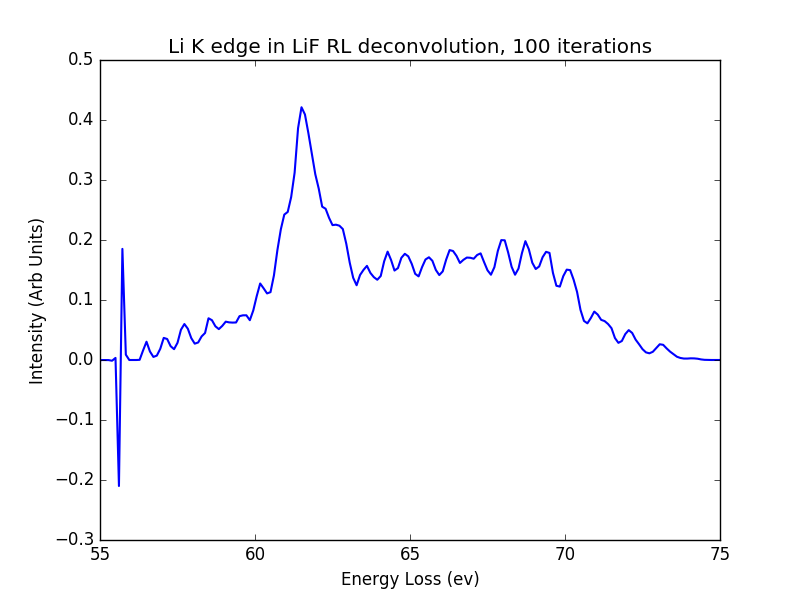
\includegraphics[scale=0.31]{/deconvolutions/100iter.png}
	\end{subfigure}

	\begin{subfigure}{0.33 \textwidth}
	\end{subfigure}

	\caption{Effect of increasing iterations in Richardson-Lucy Algorithm.  Iterations increase left to right, starting from the unprocessed background removed spectra on the top left, followed by 5, 25, 50, 100 iterations of deconvolution applied.  }
	\label{RL_iter}
\end{figure}


\subsection{Other Experimental Techniques}
EELS is not the only experimental technique available for the analysis of material microstructure, nor is it  the only electron microscopy technique available for the task. Other techniques capable of obtaining  comparable results to EELS include x-ray based analysis such as x-ray absorption spectroscopy and energy dispersive spectroscopy.  The following paragraphs briefly describe these methods and compare them to EELS.

\subsubsection{X-ray Absorption Spectroscopy (XAS)}
XAS operates on a similar principle to EELS. However, instead of probing the sample with an electron probe, a beam of x-rays is directed through the sample and like EELS the resulting energy losses in the output spectrum are binned \cite{groot_high-resolution_2001}.  This difference in probe type does not effect the measured quantity which is the same as in EELS: the unoccupied density of states of the material \cite{groot_high-resolution_2001}.  Because of their similarities, parallels have been drawn between EELS and XAS when developing theories. XAS however is typically used to measure far larger energy losses ($>$ 5 keV) and consequently has limited applicability to lithium \cite{maclaren_eels_2018}.  The most significant benefit of XAS is it's superior energy resolution ($\sim$0.1 eV) when compared to EELS ($\sim$1 eV) allowing for more features in near edge structures to be identified\cite{Egerton, groot_high-resolution_2001}.  This benefit comes at a cost however, XAS needs to be performed in a synchrotron, making it far more costly and less accessible to perform than EELS.


\subsubsection{Energy Dispersive Spectroscopy (EDS)}
EDS is another form of analytic spectroscopy performed in electron microscopy.   Unlike EELS and XAS which measure the unoccupied density of states, EDS measures the occupied DOS \cite{goldstein_electron_2003}.  Like EELS, EDS probes the sample with an electron beam, but then collects the emitted x-rays produced when the sample electrons return to their relaxed states following excitation.  These x-rays have the same characteristic energies as in EELS, but lack the resolution to distinguish fine structure.  As such, it is limited to providing only composition information on samples.  The benefit of EDS is less strict sample requirements as it does not require the thin samples needed by EELS and can therefore be used to analyze both bulk and microscale features in samples \cite{goldstein_electron_2003}.






